Even though deep learning has allowed us to do a giant leap forward on the performance of several tasks, and contrary to what some researchers claim \cite{DBLP:journals/corr/KaiserGSVPJU17}, there exists no universal model. A good model would be able to be performant in very different settings, but it won't be able to handle every situation. We need our model to be robust, but we can not expect it to be perfect. Being aware of the limitations intrinsic to the model is the best way to alleviate possible mistakes. Although it sometimes seems the case, deep learning is not a magic box, it learns from the data that we supply. If the model is biased, in all likelihood, it means that our training set is biased. In this chapter, we briefly discuss the details of implementing our method to be used in real-world setting.\\

\section{Final Model}

In the previous chapter we trained and validated several models. We found that our methodology is quite effective in the task of locating damaged buildins. We now centered our efforts in creating a final model taking into account the entire dataset of 600 tagged samples. This model was not validated as there was no images left to use as testing set. This would closely resemble a real pipeline.

We used $0.95$ as our decision threshold. According to the best of our models, this threshold guaratees us that we would have around a $0.47$ probability assigning a damaged label when the building is damaged while only having a $0.01$ probability of misslabeling a non damaged building. While this decision threshold was not necessarily valid for our final model, it gave us a hint on what decisión to make. We are sacrificing sensibility for specificity, when we predict a damage building we are confident that it will be a true positive. We could argue about the low probability of assigning a damage label but it all makes sense if we thing that we test a lot of samples for each zone.


\section{Post-processing}

So far we have centered our discussion on training a model that is able to categorize images of a particular size. Using such a model to detect collapsed buildings from the drone imagery and geolocating our findings is a completely different story. We must prost-process the information given by the model in order to tranform it into insights.

The usual methos is to use an slideing window. In this method we take a fixed window of the size that the model accepts, and we croped parts of the raster. En each step we use the model to predict on the current sample. When a prediction is positive, we save the location of the window. After the algorithm went through the whole image, we used the found positives and drew boxes over the original image. We can look at the result of this process in Figure \ref{fig:overlap}. It is evident that this approch has inherent flaws, as damaged buildings can be counted several times by the algorithm. A method to aliviate overlapping bounding boxed is known as non-maximum suppression (NMS). It was first proposed by A. Rosenfeld and M. Thurston in the context of edge detection techniques \cite{1671883}. It consist of checking the percentage of overlap in the set of bounding boxes and discarding those that repeat. The final result after postprocessing looks like Figure \ref{fig:no-overlap}.

\begin{figure}[h]
  \centering
  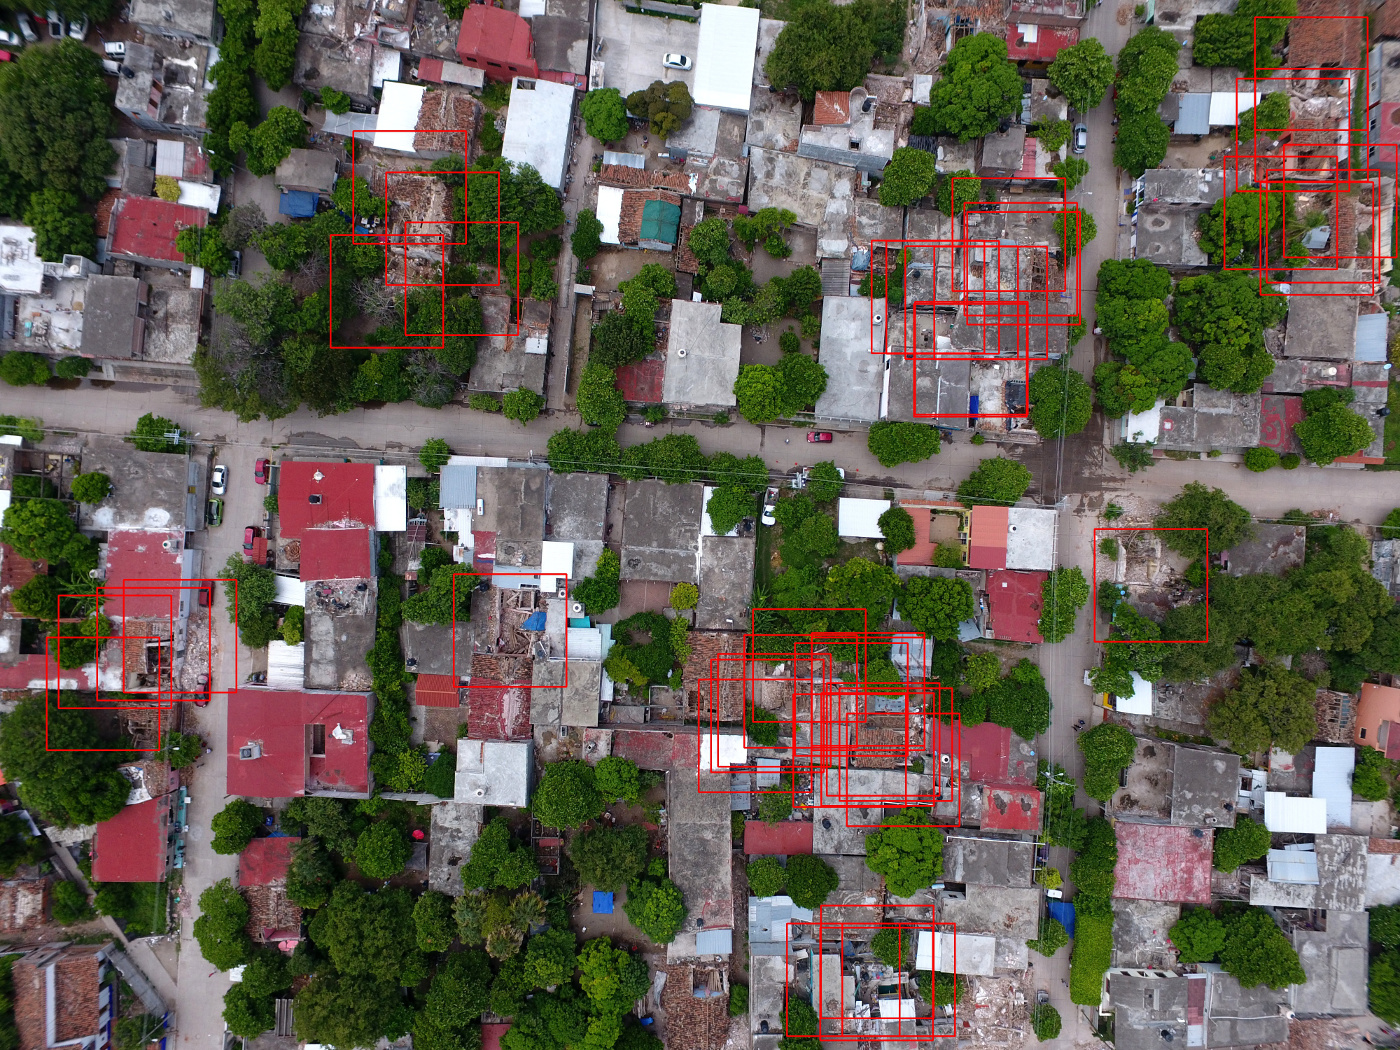
\includegraphics[width=\textwidth]{images/overlap.jpg}
  \label{fig:overlap}
  \caption{Results of our experiment. As we expected, the graph shows a positive correlation between the accuracy and the number of training samples.}
\end{figure}

\begin{figure}[h]
  \centering
  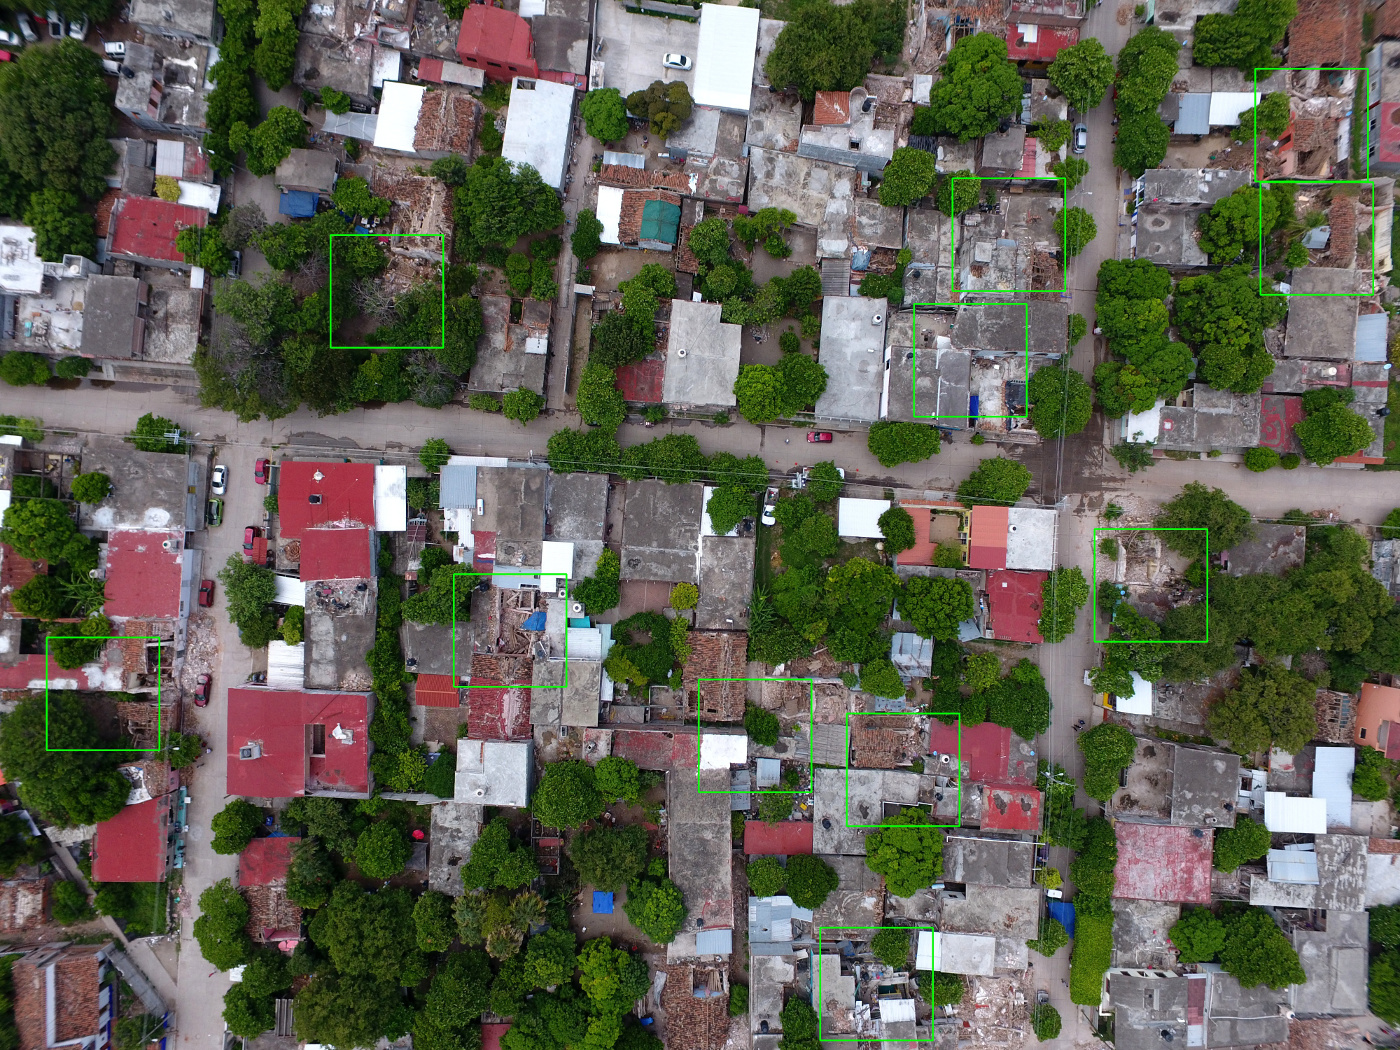
\includegraphics[width=\textwidth]{images/no-overlap.jpg}
  \label{fig:no-overlap}
  \caption{Results of our experiment. As we expected, the graph shows a positive correlation between the accuracy and the number of training samples.}
\end{figure}


\begin{figure}[h]
  \centering
  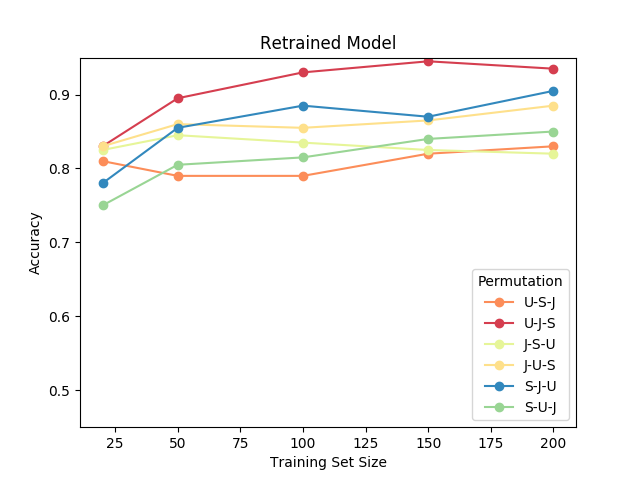
\includegraphics[width=1\textwidth]{images/validation-plot.png}
  \label{fig:validaton-plot}
  \caption{Results of our experiment. As we expected, the graph shows a positive correlation between the accuracy and the number of training samples.}
\end{figure}



\section{Deployment}

Ortorectified mosaics where built by CENAPRED using the very same images taht we used to train our models. This images come in a different format than the images taken by the drones. Additional to the optical information these tif files contain geographical location and can be used to assing a point in space to each pixel in the image. This means that we can not only locate a damaged building in an image, but to link this information with a geographical location in a given projection.\\

The images where divided in a regular grid of 299 pixel tiles with 90 pixel ovelaps. These overlaps are later postprocessed to eliminate the posibility of counting the same building twice. Each tile is exposed to the model which predicts a class on it using the previously selected threshold. When the model test a tile positive, the box is saved for postprocesing in which a technique known as non max suppression is used to eliminate boxes that represent the same object. This technique is borrowed from facial recognition algorithms. Once we have the final boxes, the center pixel of each box is transformed to world coordinates. Additionaly, this coordinates are used to query Google Maps API to obtain a human readable address for each point.\\

A shape file is produced which contains the results for each town given the output of the algorithm. This shape can be overlayed on top of the raster file using a Geographic Information System software such as QGIS. Additionaly the results are also exposed via the REST interface so they can be visualised in the web application.\\



\begin{center}
  \begin{tabular}{|c|c|c|c|c|c|}
    \hline
    town                 & positives & width & height & time (seconds) & overlap\\ \hline
    Santa Maria Xadani   &51         & 25598 & 30144  & 4420           & 0.1 \\ \hline
    Juchitan de Zaragoza &302        & 42375 & 28831  & 6375           & 0.1 \\ \hline
    Union Hidalgo        &25         & 19945 & 28795  & 3938           & 0.1\\
    \hline
  \end{tabular}
\end{center}


